\documentclass{article}
\usepackage{amsmath}
\usepackage{hyperref}
\usepackage{graphicx}
\usepackage{adjustbox}
\usepackage{caption}
\usepackage{subfigure}
\newcommand{\tabincell}[2]{\begin{tabular}{@{}#1@{}}#2\end{tabular}}
\begin{document} %This is where document begins
\begin{titlepage}
\title{EE 232E \\Graphs and Network Flows\\Project 1\\Winter 2016} 
\author{Liqiang Yu, Rongjing Bai, Yunwen Zhu\\
904592975, 204587519, 104593417}  %change your ID here
\date{05-14-2016}
\end{titlepage}
\maketitle
\newpage
\tableofcontents
\newpage
\section{Problem 1}
We read the txt file and construct the graph.
After we constructed the graph, we found that the graph is connected.\\
The diameter is 8.\\
Intuitively, we believer that the distribution should be $$\frac{1}{y} \sim a*x^{p}+b$$\\
which means frequency should be inverse proportional  to $a*degree^{p}+b$\\
After fitting the data, the coeficient is a=0.042,b=40.39,p=2.065\\
So the model is $$y=\frac{1}{0.042*x^{2.065}+40.39}$$
The MSE for this model is $2.6*10^{-1}$
The average degree is 43.691.
\section{Problem 2}
We constructed the graph shown in figure. The graph has 2866 edges and 348 nodes in total.
\section{Problem 3}
We can find the neighbors of certain node by neighborhood() function. Then we find the core nodes with more than 200 neighbors.There are 40 core nodes in total, and their average degree is 279.375.
To analyze the personal network, we choose node 1 as the core node. We can see the personal network of node 1 from the figure \ref{fig:p3_1}.
\ref{fig:p3_1}
\begin{figure}[htbp]
\centering
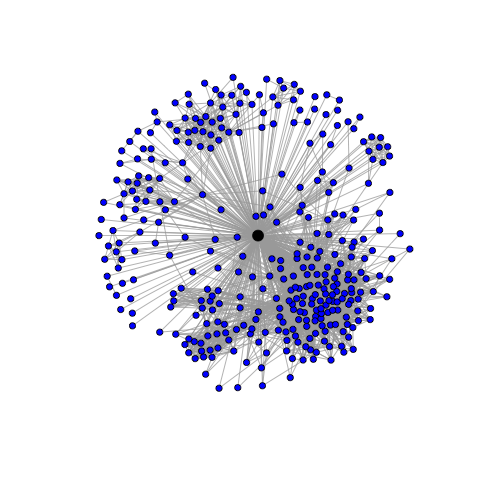
\includegraphics[width=.8\textwidth]{3_1.png}
\caption{Personal Network of core node 1}
\label{fig:p3_1}
\end{figure}
In this part, we use Fast-Greedy, Edge-Betweenness, and Infomap community these three algorithms in igraph to find out the community structure of the personal network of node 1. 
We can get three different community structure detection results from the graph pairs shown below. In each graph pair, the left subgraph shows the partition results of the community, which are distinguished by different colors. The core nodes in the subgraph are highlighted with larger size. The right subgraph shows the community distribution of the network.\\
\\
\begin{figure}[htbp]
\centering
%\captionsetup{justification=centering,margin=2cm}

\subfigure{
\begin{minipage}[b]{0.4\textwidth}
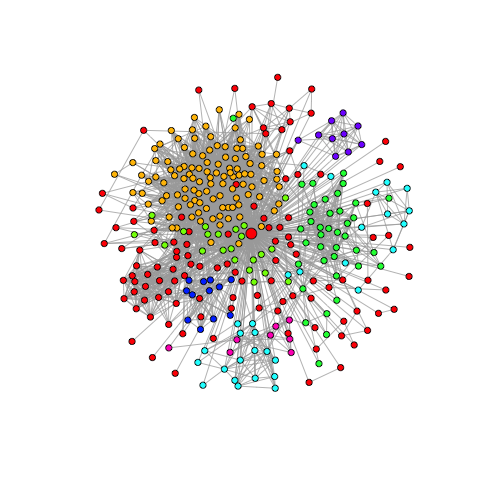
\includegraphics[width=1\textwidth]{3_2.png} \\
\caption*{The community structure for fast-greedy method}
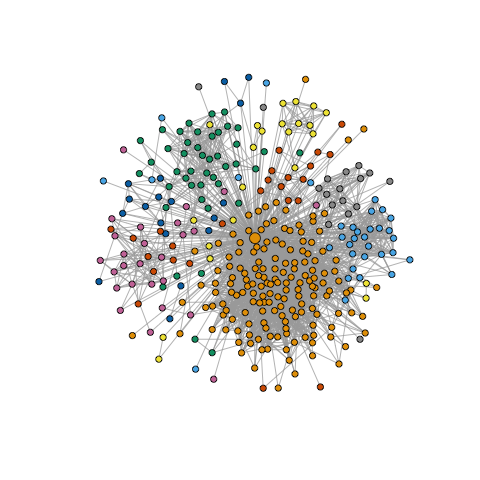
\includegraphics[width=1\textwidth]{3_4.png}\\
\caption*{The community structure for edge-betweenness method}
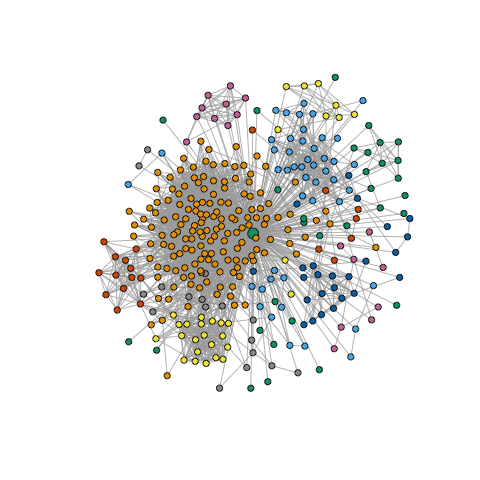
\includegraphics[width=1\textwidth]{3_6.png}
\caption*{The community structure for infomap method}
\end{minipage}
}
\subfigure{
\begin{minipage}[b]{0.4\textwidth}
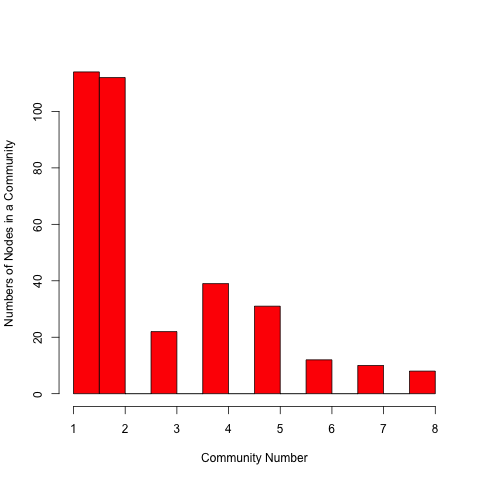
\includegraphics[width=1\textwidth]{3_3.png} \\
\caption*{Community distribution for fast-greedy method}
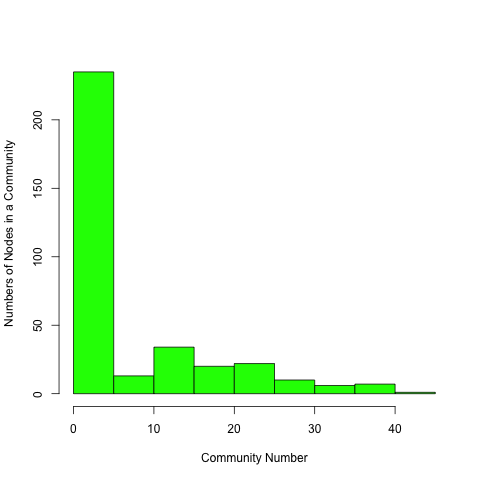
\includegraphics[width=1\textwidth]{3_5.png}\\
\caption*{Community distribution for edge-betweenness method}
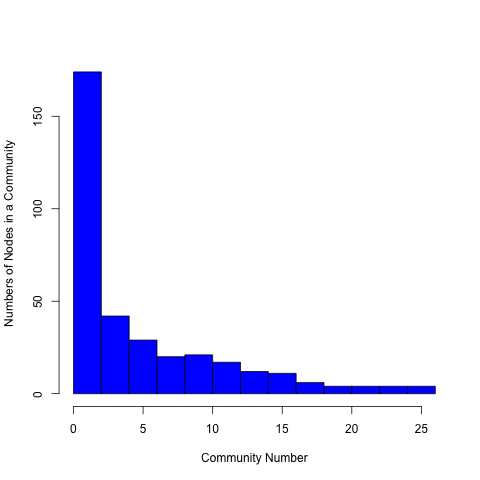
\includegraphics[width=1\textwidth]{3_7.png}
\caption*{Community distribution for infomap method}
\end{minipage}
}
\caption{}

\label{fig:p3_2}
\end{figure}
\noindent Based on the results of three community detection algorithms, we can find out that there are some differences such as modularity and number of communities besides the community structure. The result is shown in table \ref{tb:p3}.
\begin {table}[htbp]
\caption{The modularity and number of communities comparison results}
\begin{adjustbox}{center}
\label{tb:p3}
\begin{tabular}{|c|c|c|c|}
\hline
&fast-greedy &edge-betweenness &infomap\\
\hline
modularity&0.4131014&0.3533022&0.3891184\\
\hline
number of communities&8&41 & 26\\
\hline
\end{tabular}
\end{adjustbox}
\end{table}
From the result we can see that these three algorithms have similar modularities, but have great difference in community numbers. Fast-Greedy has the coarsest clusters, while Edge-Betweenness is the finest. However, from figure\ref{fig:p3_2} shows several communities in Edge-Betweenness are actually composed by single node, i.e., these nodes do not have tight connection with other nodes in the network. Thus, the modularity of Edge-Betweenness is relatively lower than that of Fast-Greedy and Infomap.


\section{Problem 4}
After deleting the core node 1, the personal network of core node 1 is shown in figure \ref{fig:p4_1}
\begin{figure}[htbp]
\centering
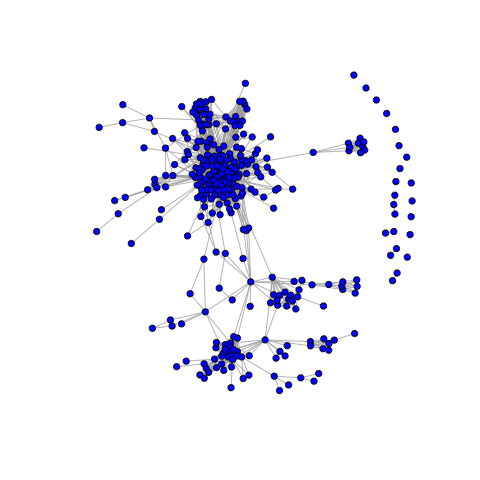
\includegraphics[width=.8\textwidth]{p4_1.png}
\caption{in degree distribution}
\label{fig:p4_1}
\end{figure}
After applying Fast Greedy, Edge Betweenness and Infomap algorithms to the personal network of core node 1 after the deletion, we can explore the community structures and compare them with the network before the deletion. The results are shown in figure \ref{fig:p4_2}. The left column are the community structures after applying three kinds of algorithms and the right column are the comparison results of the community distribution before and after the deletion.\\
\\
 From figure \ref{fig:p4_2} we can see that edge betweenness and infomap method almost produced the same results, but fast greedy produced the distribution that moved right a little bit. \\
 \\
 Moreover, the modularity results before and after the deletion are shown in table \ref{tb:p4}. From the results we can see that infomap produced exactly the same results, however fast greedy and edge betweenness both produced larger results after the deletion, which makes sense. Because the modularity is, quoted from wikipedia, "designed to measure the strength of division of a network into modules (also called groups, clusters or communities). Networks with high modularity have dense connections between the nodes within modules but sparse connections between nodes in different modules." After deleting the core node, which is pivot node of the its personal network, the network should be easier to divide into modules and therefore the modularity should increase.
\begin{figure}[htbp]
\centering
%\captionsetup{justification=centering,margin=2cm}

\subfigure{
\begin{minipage}[b]{0.4\textwidth}
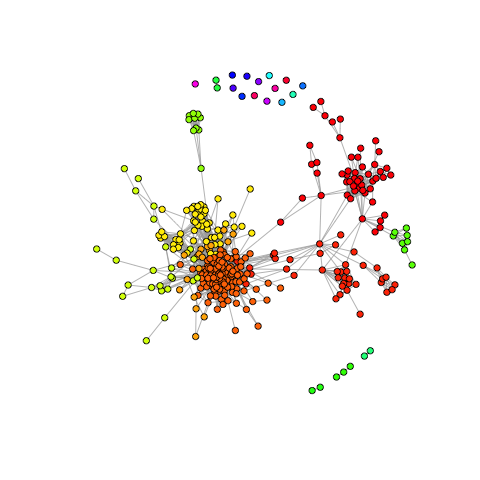
\includegraphics[width=1\textwidth]{p4_2_fgc.png} \\
\caption*{The community structure for fast-greedy method}
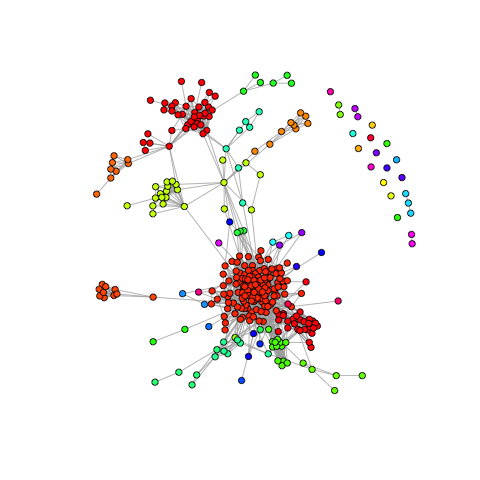
\includegraphics[width=1\textwidth]{p4_2_ebc.png}\\
\caption*{The community structure for edge-betweenness method}
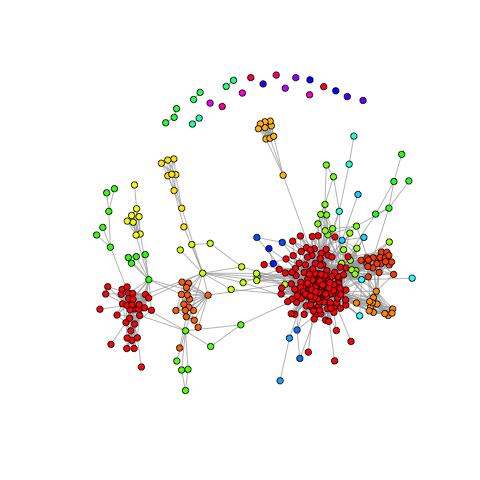
\includegraphics[width=1\textwidth]{p4_2_ifc.png}
\caption*{The community structure for infomap method}
\end{minipage}
}
\subfigure{
\begin{minipage}[b]{0.4\textwidth}
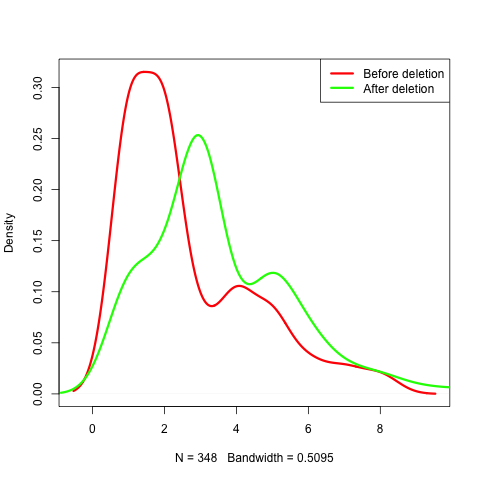
\includegraphics[width=1\textwidth]{density_compare_fgc.png} \\
\caption*{The comparison results for fast-greedy method}
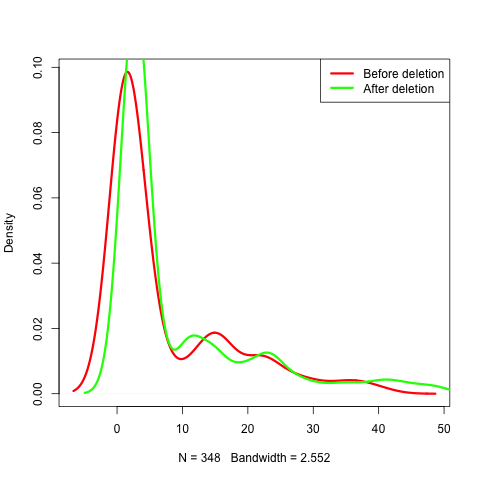
\includegraphics[width=1\textwidth]{density_compare_ebc.png}\\
\caption*{The comparison results for edge-betweenness method}
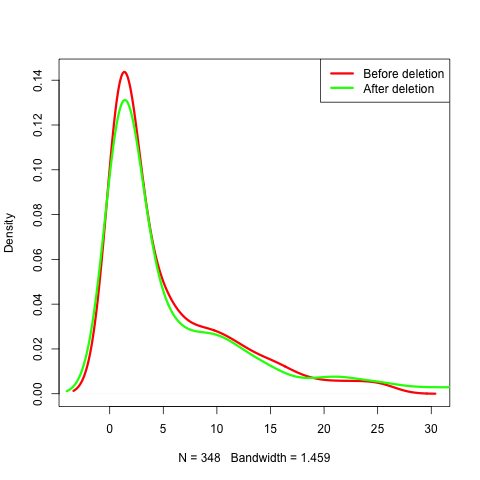
\includegraphics[width=1\textwidth]{density_compare_ifc.png}
\caption*{The comparison results for infomap method}
\end{minipage}
}
\caption{}
\label{fig:p4_2}
\end{figure}

\begin {table}[htbp]
\caption{The modularity comparison results}
\begin{adjustbox}{center}
\label{tb:p4}
\begin{tabular}{|c|c|c|c|}
\hline
&fast-greedy &edge-betweenness &infomap\\
\hline
Before deletion&0.4131014&0.3533022&0.3891184\\
\hline
After deletion&0.4418533& 0.4161461& 0.4180077\\
\hline
\end{tabular}
\end{adjustbox}
\end{table}

\section{Problem 6}
In this problem, we choose to use the cluster coefficient and density to define two types of communities in the 41 personal networks. We try to find the community indices that have maximal and minimal results and compare them to draw the conclusion.
\subsection{Clustering Coefficient}
\subsubsection{Global Clustering Coefficient}
The global clustering coefficient is based on triplets of nodes. A triplet consists of three connected nodes. A triangle therefore includes three closed triplets. Therefore the global clustering coefficient is the number of closed triplets (or 3 x triplets) over the total number of triplets.
\begin{equation*}
C = \frac{3\;\times\;number\; of\; triangles}{number\; of\; connected\; triplets}
\end{equation*}
\subsubsection{Local Clustering Coefficient}
The local clustering coefficient of a vertex in a graph quantifies how close its neighbors are to being a clique. A graph $G=(V,E)$ formally consists of a set of vertices $V$ and a set of edges $E$ between them. A edge $e_{ij}$ connects vertex $v_i$ with $v_j$. The neighborhood $N_i$ for a vertex $v_i$ is defined as its immediately connected neighbors as follows
\begin{equation*}
N_i=\lbrace v_j:e_{ij}\in E \cup e_{ji} \in E \rbrace
\end{equation*} 
we define $k_i$ as the number of vertices in $N_i$. So the local clustering coefficient for undirected graph is
\begin{equation*}
C_i = \frac{2 \vert \lbrace e_{jk} : v_j, v_k \in N_i, e_{jk} \in E\rbrace\vert}{k_i(k_i-1)}
\end{equation*}
\subsubsection{Network average clustering coefficient}
As an alternative to the global clustering coefficient, the overall level of clustering in a network is measured as the average of the local clustering coefficients of all the vertices $n$
\begin{equation*}
\bar{C} = \frac{1}{n} \sum_{i=1}^nC_i
\end{equation*}
\subsection{Density} 
Network density describes the portion of the potential connections in a network that are actual connections. A potential network is a connection that could potentially exist between two nodes - regardless of whether or not it actually does. That is, for a cluster $c$, the density $d(c)$ is defined as\\
\begin{equation*}
d(c) = \frac{2 \times E(c)}{|c|(|c|-1)}
\end{equation*}
where $E(c)$ is the number of edges in cluster $c$ and $|c|$ is the number of vertices in cluster $c$.
High density means there are dense connections inside the cluster therefore a network with high density has large possibility to be a clique.
\subsection{Resutls}
The results are shown in table \ref{tb:type}. We calculate both the cluster coefficient and density of each community that is larger than 10 in each personal network and store the community indices of the largest and smallest values.\\
\begin{table}[hbp]
\caption{The two type communities' indices}
\begin{adjustbox}{center}
\label{tb:type}
\begin{tabular}{|c|c|}
\hline
type1 cluster &6 3 2 4 1 1 1 2 1 2 1 1 2 2 2 2 1 3 2 1 1 1 2 3 1 2 1 2 3 2 3 1 1 2 1 1 2 1 2 1 2\\
\hline
type1 density &6 3 2 4 1 1 1 2 1 2 1 1 2 2 2 2 1 3 2 1 1 1 2 3 1 2 1 2 3 2 3 1 1 2 1 1 2 1 2 1 2\\
\hline
type2 cluster &7 4 3 5 4 3 2 1 3 1 2 3 1 1 1 1 2 1 3 2 8 2 1 1 2 1 2 1 1 1 1 2 2 1 2 2 1 2 1 2 1\\
\hline
type2 density &7 4 3 5 4 3 2 1 3 1 2 3 1 1 1 1 2 1 3 2 8 2 1 1 2 1 2 1 1 1 1 2 2 1 2 2 1 2 1 2 1\\
\hline
\end{tabular}
\end{adjustbox}
\end{table}
\\
Type 1 are indices with largest values and type 2 are indices with smallest values. From the table \ref{tb:type} we can see that clustering coefficient and density gave exactly the same results. So we can draw the conclusion that both clustering coefficient and density can distinguish two types of communities, one is densely connected inside, maybe a network of high school classmates and another sparselyl connected inside, maybe the fans of a sport team.


\section{Problem 7}
In this problem, we analyze Google+ with tagged relationships. Since the core node is not available in the edgelist, we first manually add the ego node and all the corresponding edges into the graph. After exporting the whole network, we can use Walktrap and Infomap algorithms to find the community structure, and we randomly choose to plot the ego node 2's community structure for Walktrap and Infomap algorithm in figure \ref{fig:p7_1}.\\
\\

\begin{figure}[htbp]
\centering
%\captionsetup{justification=centering,margin=2cm}

\subfigure{
\begin{minipage}[b]{0.4\textwidth}
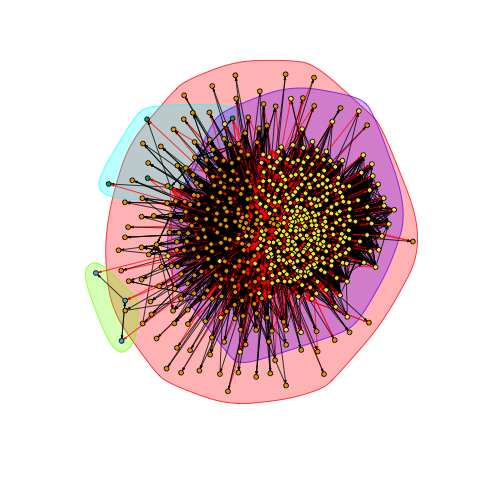
\includegraphics[width=1\textwidth]{7_1.png} \\
\caption*{The community structure for walktrap method of ego node 2}
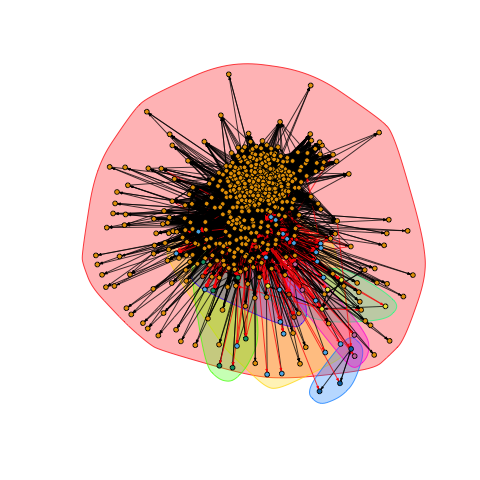
\includegraphics[width=1\textwidth]{7_2.png}\\
\caption*{The community structure for infomap method of ego node 2}
\end{minipage}
}
\subfigure{
\begin{minipage}[b]{0.4\textwidth}
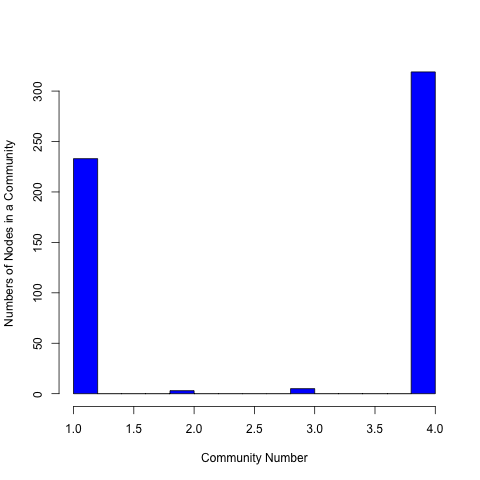
\includegraphics[width=1\textwidth]{7_3.png} \\
\caption*{community distribution for walktrap method of ego node 2}
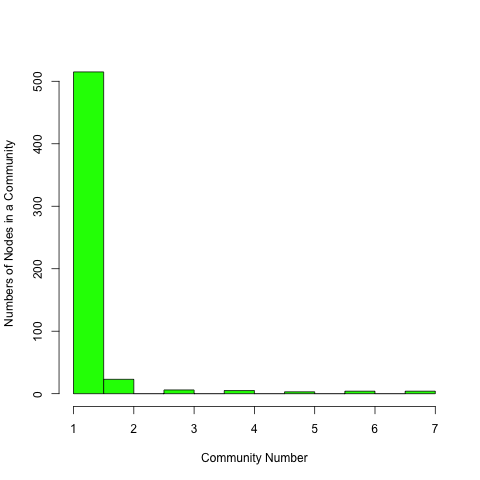
\includegraphics[width=1\textwidth]{7_4.png}\\
\caption*{community distribution for infomap method of ego node 2}
\end{minipage}
}
\caption{community structure}
\label{fig:p7_1}
\end{figure}

\noindent To analyze the communities' overlap with the users' circle, we use the Balanced Error Rate(BER) between the community and the tagged circles. We define the community detected by community detection algorithm as $C=\{C_1,...,C_K \}$ and tagged circle as $C'=\{C'_1,...,C'_K\}$ .
\begin{equation*}
BER(C,C') = \frac{|C\backslash C'|}{2|C|} + \frac{|C^c\backslash C'^c|}{2|C^c|}
\end{equation*}
\\
Then we use this equation to compute each community and circle's match to find the most matched circle for each community. $\lambda$ = 1 - BER,  the $\lambda$indicates the overlap between each community and circles, i.e the larger $\lambda$ the community has with a circle, the closer this circle is with the community.On the basis of matching circle for each community, we calculate the number of nodes within the overlap area as well as the number of nodes located outside the circle to get the corresponding overlapping level.\\
\\
Moreover our analysis is based on two assumptions:
(1) The division of community is based on the connectivity of each pair of nodes, thus it is objec- tive. However, the tagging of users are relatively subjective and inconsistent, because it depends on user. So we should use communities to measure circles, not vice versa.
(2) Each node can belong to multiple circles, but only one community. So it is more feasible and rational to measure by community.
\\
The results of communities overalp with circles in the two detected algorithms are shown in figure
\ref{fig:p7_2} and \ref{fig:p7_3}.

\begin{figure}[htbp]
\centering
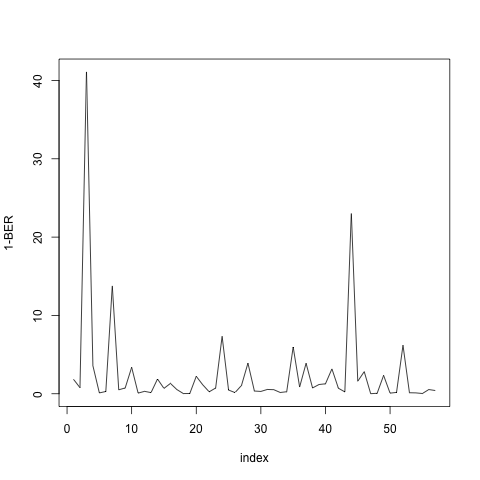
\includegraphics[width=.8\textwidth]{7_5.png}
\caption{overlap on communities for walktrap method}
\label{fig:p7_2}
\end{figure}

\begin{figure}[htbp]
\centering
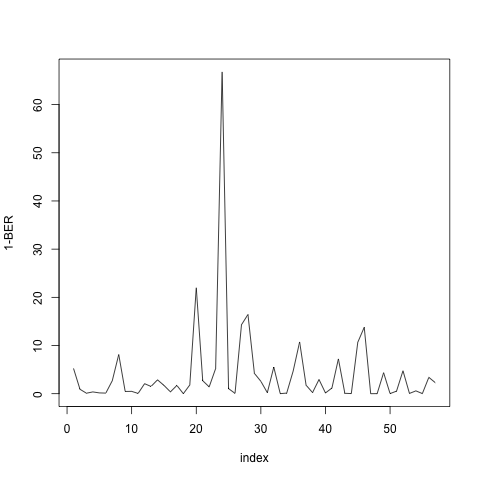
\includegraphics[width=.8\textwidth]{7_6.png}
\caption{overlap on communities for infomap method}
\label{fig:p7_3}
\end{figure}
\noindent From the figure above, we can see that there are some high overlaps among certain users. That means the user tags one person into the circle where there are the majority of members of that community, then this tagging fits the community structure. Thus, it is highly dependent on user's habit on tagging relationships with circles.
\end{document}